\chapter{About the Author}

\begin{figure}[h]
  \centering
  \fbox{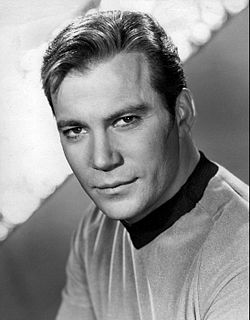
\includegraphics[totalheight=3in,natwidth=250,natheight=320]{frontmatter/about-author/media/james-t-kirk}}
  \caption{James Tiberius Kirk}
\end{figure}

James Tiberius ``Jim'' Kirk is a fictional character in the Star Trek media franchise, appearing in numerous television episodes, films, books, comics, and video games. As the captain of the starship USS Enterprise, Kirk leads his crew as they explore ``where no man has gone before''.

Kirk, played by William Shatner, first appears in the broadcast pilot episode of Star Trek: The Original Series, ``The Man Trap'', originally broadcast on September 8, 1966. Shatner continued in the role for the show's three seasons, and later provided the voice of the animated version of Kirk in Star Trek: The Animated Series (1973–74). Shatner returned to the role for Star Trek: The Motion Picture (1979) and in six subsequent films. Chris Pine portrays a young version of the character in the 2009 reboot Star Trek film, with Jimmy Bennett playing Kirk as a child. Other actors have played the character in fan-created media, and the character has been the subject of multiple spoofs and satires.

The character is primarily a protagonist in the media in which he appears, often with the characters of Spock and Leonard McCoy acting as logical and emotional sounding boards, respectively. The character has been praised for his leadership traits, and also criticized for his relationships with women.

All information is from wikipedia\footnote{http://en.wikipedia.org/wiki/James\_T.\_Kirk}